\documentclass[xetex,serif]{beamer}
%\usepackage[driver=xetex,a4paper,left=35mm,right=35mm,top=30mm,bottom=40mm]{geometry} % propper margins on a4 paper
%\usepackage{url}
%\usepackage[hidelinks]{hyperref} % make contents and references clickable in pdf
\usepackage[english]{babel}
\usepackage[english]{isodate} \isodate%
\usepackage[absolute,overlay]{textpos}
\usepackage{graphicx} % include images
\usepackage{pgfplots}
\graphicspath{{graphics/}}

\usepackage{fontspec} % allows custom fonts
\setmainfont[BoldFont=Source Sans Pro Bold,AutoFakeSlant=0.3]{Source Serif Pro}
\setmonofont{Source Code Pro}

\usetheme{default}
\usecolortheme{crane}

\beamertemplatenavigationsymbolsempty
%\setbeamercolor{footline}{fg=black}
%\setbeamerfont{footline}{size=\normalsize}
%\addtobeamertemplate{navigation symbols}{}{%
%    \usebeamerfont{footline}%
%    \usebeamercolor[fg]{footline}%
%    \hspace{1em}%
%    \insertframenumber
%}

\title{Design and implementation of the\\Meta Casanova 3 compiler back-end}
\author{Douwe van Gijn}
\date{2016-06-29}

\begin{document}
{%
%\setbeamertemplate{footline}{}%
\begin{frame}[noframenumbering]%
\titlepage%
\end{frame}%
}

\begin{frame}\frametitle{Introduction}
\begin{itemize}
    \item games
\end{itemize}

\end{frame}\begin{frame}\frametitle{Research question}
\textit{How to implement a transformation from typechecked Meta Casanova from the front-end, to executable code within the timeframe of the internship?}

\end{frame}\begin{frame}\frametitle{Requirements}
    
\begin{itemize}
    \item The correctness requirement
    \item The .NET requirement
    \item The multiplatform requirement
    \item The performance requirement
\end{itemize}

\end{frame}\begin{frame}[t]\frametitle{Sub-questions}
\begin{itemize}
    \item The language question
    \item The interface question
    \item The IR question
    \item The codegen question
    \item The mangle question
    \item The validation question
    \item The debug question
\end{itemize}
\begin{textblock*}{0.75\paperwidth}(0.125\paperwidth,6cm)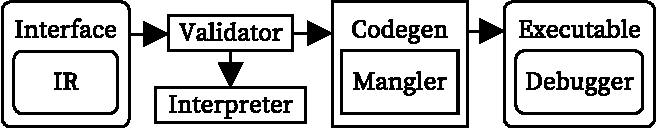
\includegraphics[width=0.75\paperwidth]{overview}\end{textblock*}

\end{frame}\begin{frame}[t]\frametitle{The language question}
\begin{textblock*}{0.75\paperwidth}(0.125\paperwidth,6cm)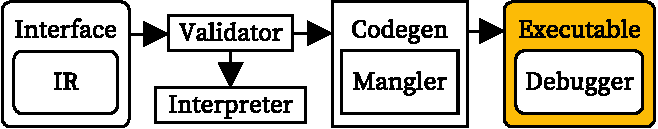
\includegraphics[width=0.75\paperwidth]{overview_language}\end{textblock*}

\end{frame}\begin{frame}[t]\frametitle{The interface question}
\begin{textblock*}{0.75\paperwidth}(0.125\paperwidth,6cm)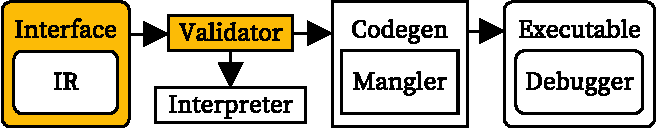
\includegraphics[width=0.75\paperwidth]{overview_interface}\end{textblock*}

\end{frame}\begin{frame}[t]\frametitle{The IR question}
\begin{textblock*}{0.75\paperwidth}(0.125\paperwidth,6cm)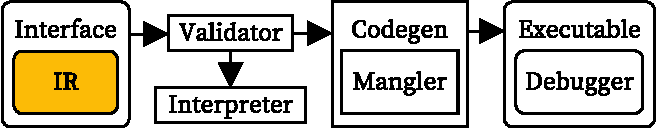
\includegraphics[width=0.75\paperwidth]{overview_ir}\end{textblock*}

\end{frame}\begin{frame}[t]\frametitle{The codegen question}
\begin{textblock*}{0.75\paperwidth}(0.125\paperwidth,6cm)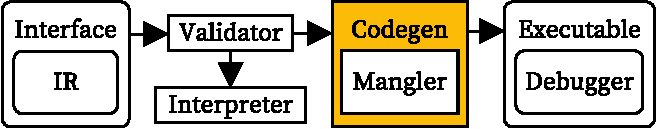
\includegraphics[width=0.75\paperwidth]{overview_codegen}\end{textblock*}

\end{frame}\begin{frame}[t]\frametitle{The mangle question}
\begin{textblock*}{0.75\paperwidth}(0.125\paperwidth,6cm)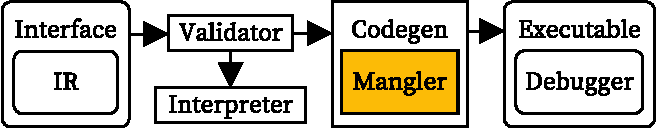
\includegraphics[width=0.75\paperwidth]{overview_mangler}\end{textblock*}

\end{frame}\begin{frame}[t]\frametitle{The validation question}
\begin{textblock*}{0.75\paperwidth}(0.125\paperwidth,6cm)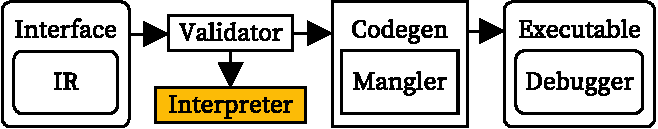
\includegraphics[width=0.75\paperwidth]{overview_validation}\end{textblock*}

\end{frame}\begin{frame}[t]\frametitle{The debug question}
\begin{textblock*}{0.75\paperwidth}(0.125\paperwidth,6cm)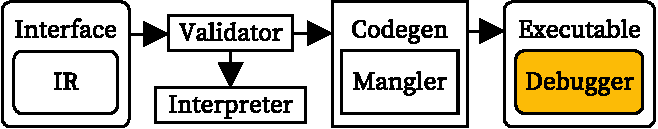
\includegraphics[width=0.75\paperwidth]{overview_debugger}\end{textblock*}

\end{frame}\begin{frame}\frametitle{Results}
\begin{itemize}
    \item The correctness requirement
    \item The .NET requirement
    \item The multiplatform requirement
    \item The performance requirement
\end{itemize}

\end{frame}\begin{frame}\frametitle{The correctness \& .NET requirement}
    Test programs

\end{frame}\begin{frame}\frametitle{The multiplatform requirement}
    Microsoft .NET Compiler for windows

    Mono everywhere else

\end{frame}\begin{frame}\frametitle{The performance requirement}
\begin{tikzpicture}
\begin{axis}[
        symbolic x coords={Min, Avg, Max},
        xtick=data,
	x tick label style={},
        ylabel=time ($\mu$s),
	enlargelimits=0.2,
        grid=major,
	legend style={at={(1.1,0.5)},
	anchor=west,legend columns=1},
	ybar,
]
\addplot[black,fill=gray]   coordinates {(Min,39.00) (Avg,41.95) (Max,52.86)};
\addplot[black,fill=craneorange] coordinates {(Min,22.82) (Avg,36.30) (Max,49.79)};
\legend{Python,MC}
\end{axis}
\end{tikzpicture}

\end{frame}\begin{frame}\frametitle{Conclusion}
\begin{itemize}
    \item All requirements are met
    \item Working back-end within the allocated time
    \item Demo time!
\end{itemize}

\end{frame}\begin{frame}\frametitle{Defence}
    Come at me!

\end{frame}
\end{document}
